\documentclass[xcolor=pdftex,dvipsnames,table,mathserif,aspectratio=169]{beamer}
\usetheme{metropolis}

%\usetheme{Darmstadt}
%\usepackage{times}
%\usefonttheme{structurebold}

\usepackage[english]{babel}
%\usepackage[table]{xcolor}
\usepackage{pgf,pgfarrows,pgfnodes,pgfautomata,pgfheaps}
\usepackage{amsmath,amssymb,setspace,centernot}
\usepackage[latin1]{inputenc}
\usepackage[T1]{fontenc}
\usepackage{relsize}
\usepackage{stmaryrd}
\usepackage{pdfpages}
\usepackage{booktabs}
\usepackage[absolute,overlay]{textpos} 


\newenvironment{reference}[2]{% 
  \begin{textblock*}{\textwidth}(#1,#2) 
      \footnotesize\it\bgroup\color{red!50!black}}{\egroup\end{textblock*}} 

\DeclareMathSizes{10}{10}{6}{6} 
\AtBeginSection[]{
  \begin{frame}
  \vfill
  \centering
  \begin{beamercolorbox}[sep=8pt,center,shadow=true,rounded=true]{title}
    \usebeamerfont{title}\insertsectionhead\par%
  \end{beamercolorbox}
  \vfill
  \end{frame}
}
\begin{document}
\title{Conduct}
\author{Chris Conlon}
\institute{Grad IO}
\date{\today}

\frame{\titlepage}

\begin{frame}{Conduct Overview}
\begin{itemize}
\item A second set of important questions in IO is being able to use data to decide whether firms are \alert{competing} or \alert{colluding}.
\item Absent additional restrictions, we cannot generally look at data on $(P,Q)$ and decide whether or not collusion is taking place.
\begin{itemize}
\item You say we started colluding at date $t$, I say we received a correlated shock to $mc$.
\end{itemize}
\item We can make progress in two ways: (1) parametric restrictions on marginal costs; (2) exclusion restrictions on supply.
\begin{itemize}
\item Most of the literature focuses on (1) by assuming something like: $\ln mc_{jt} = x_{jt} \gamma_1 + w_{jt} \gamma_2 + \omega_{jt}$.
\item In principle (2) is possible if we have instruments that shift demand for products but not supply. (These are much easier to come up with than ``supply shifters'').
\end{itemize}
\end{itemize}
\end{frame}

\begin{frame}{A famous plot (Bresnahan 87)}
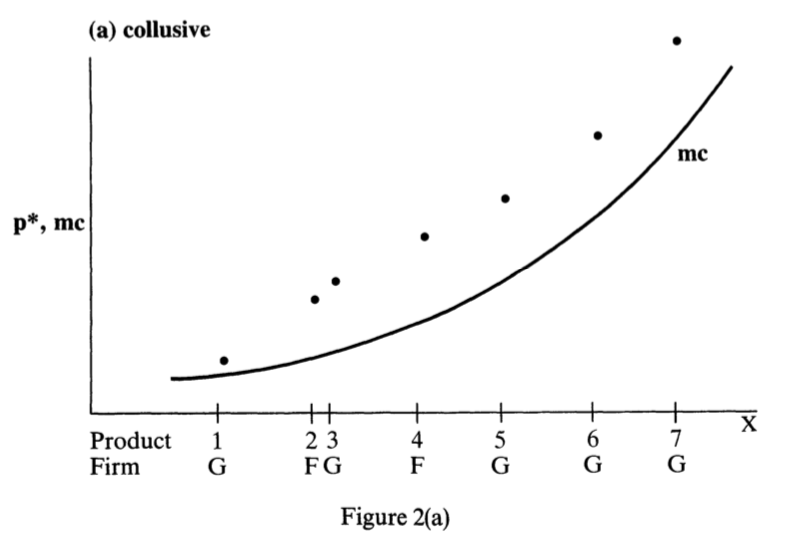
\includegraphics[width = 6.6cm]{./resources/bres_plot1.png}
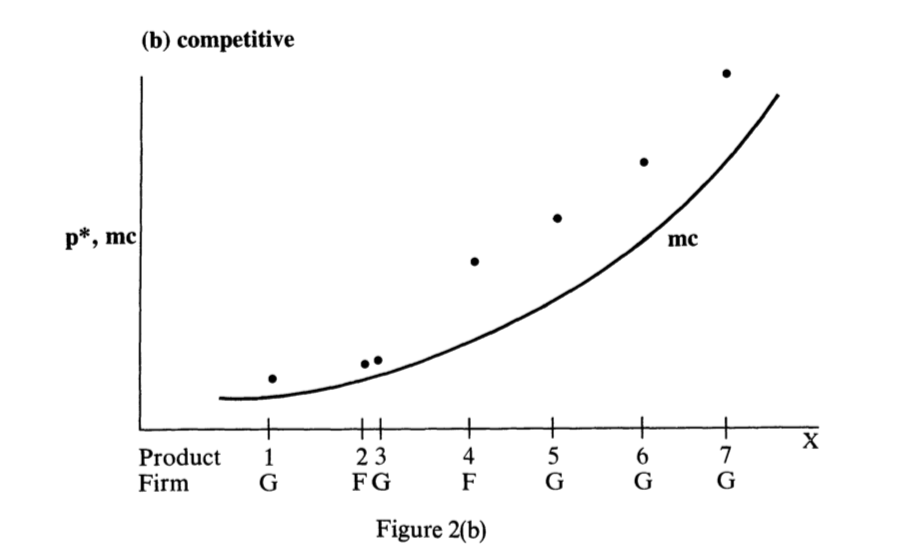
\includegraphics[width = 6.9cm]{./resources/bres_plot2.png}\\
Bresnahan (1980/1982) recognized this problem: we need ``rotations of demand''.
\end{frame}


\begin{frame}
\frametitle{Testing For Collusion: Challenges}
\small
We generalize the $\mathcal{H}(\kappa)$ and derive multi-product Bertrand FOCs:
\begin{align*}
\arg \max_{p \in \mathcal{J}_f} \pi_f (\mathbf{p}) &= \sum_{j \in \mathcal{J}_f} (p_j - c_j) \cdot q_j(\mathbf{p}) +  \alert{\kappa_{fg} \sum_{j \in \mathcal{J}_g} (p_j - c_j) \cdot q_j(\mathbf{p})} \\
\rightarrow 0&= q_j(\mathbf{p}) + \sum_{k \in (\mathcal{J}_f,\mathcal{J}_g)} \alert{\kappa_{fg}}\cdot (p_k - c_k) \frac{\partial q_{k}}{\partial p_j}(\mathbf{p}) 
\end{align*}
\begin{itemize}
\item Instead of $0$'s and $1$'s we now have $\kappa_{fg} \in [0,1]$ representing how much firm $f$ cares about the profits of $g$.
\begin{itemize}
\item If $f$ and $g$ merge (or fully colluded) then $\kappa_{fg} =1$
\item Often in the real world firms cannot reach fully collusive profits and $\kappa_{fg} \in (0,1)$.
\item Evidence that $\kappa_{fg} > 0$ is not necessarily evidence of malfeasance, just a deviation from \alert{static Bertrand pricing}
\end{itemize}
\end{itemize}
\end{frame}


\begin{frame}{Testing For Conduct: Challenges}
\begin{itemize}
\item Recall the $\Delta$ matrix which we can write as $\Delta=\tilde{\Delta}\, \odot \mathcal{H}(\kappa)$, where $\odot$ is the element-wise or Hadamard product of two matrices. 
\begin{itemize}
\item $\tilde{\Delta}$ is the matrix of demand derivatives with $\Delta{(j,k)} = \frac{\partial q_j}{\partial p_k}$ for all elements.
\item $\mathcal{H}(\kappa)=\kappa_{fg}$ for products owned by $(f,g)$ where $\kappa_{ff}=1$ always.
\end{itemize}
\item Mergers are about changing $0$'s to $1$'s in the $\mathcal{H}(\kappa)$ matrix.
\item Matrix form of FOC: $q(\mathbf{p}) = \Delta(\mathbf{p},\kappa)\cdot(\mathbf{p}-\mathbf{mc})$
\item $\mathbf{mc} =  \mathbf{p} - \underbrace{\Delta(\mathbf{p}, \theta_2, \kappa)^{-1} s(\mathbf{p})}_{\eta(\mathbf{p},\mathbf{s},\theta_2,\kappa)}$
where $\eta_{jt}$ is the markup.
\end{itemize}
\end{frame}

\begin{frame}
\frametitle{Reasons for Deviations from Static Bertrand}
\small
\begin{description}
\item[Biased estimates of own and cross price derivatives:] For anything to work, you have correct estimates of $\tilde{\Delta}$. My prior is most papers \alert{underestimate} diversion ratios for close substitutes.
\item[Vertical Relationships:] Who sets supermarket prices? Just the retailer? Just the manufacturer? Some combination of both? Retailers tend to \alert{soften} downstream price competition.
\item[Faulty Timing Assumptions:] Bertrand is a simultaneous move pricing game. Lots of alternatives (Stackelberg leader-follower, Edgeworth cycles, etc.).
\item[Dynamics and Dynamic Pricing:] Forward looking firms or consumers might not set static Nash prices. [e.g. Temporary Sales, Switching Costs, Network Effects, etc.]
\item[Unmodeled Supergame:] Maybe firms are legally tacitly colluding, higher prices might be about what firms believe will happen in a price war.
\end{description}
\end{frame}


\begin{frame}{Simultaneous Problem}
Assume additivity, and write in terms of structural errors:
\begin{align*}
\delta_{jt}(\mathcal{S}_t,\widetilde{\theta}_2) + \alpha p_{jt} &= h_d(x_{jt}, \, \alert{v_{jt}},\theta_1)  + \xi_{jt} \\
 f \left( p_{jt} - \eta_{jt}(\mathbf{p},\mathbf{s},\theta_2,\kappa) \right) &= h_s(x_{jt}, \alert{w_{jt}},\theta_3) + \omega_{jt}
\end{align*}
\vspace{-.4cm}
\begin{itemize}
\item To simplify slides we let $f(x)=x$ (often $f(x) =\log(x))$.
\item $h(\cdot)$ are often just linear relationships $\theta_1 [x_{jt}, v_{jt}]$.
\item $(\theta_2, \kappa)$ parameters are what determine markups
\item so does $(\xi,\omega)$ through 
\end{itemize}
\end{frame}


\begin{frame}
\frametitle{Approach \#1: Demand Side}
1. Estimate $\theta_2$ from demand alone.
\begin{align*}
\delta_{jt}(\mathcal{S}_t,\widetilde{\theta}_2) + \alpha p_{jt} &= h_d(x_{jt}, \, \alert{v_{jt}},\theta_1)  + \xi_{jt} \\
E[\xi_{jt} | x_{t}, v_{t}, w_{t}] &=0
\end{align*}
2. Recover marginal costs $\widehat{\mathbf{mc}} = \mathbf{p} +(\mathcal{H}(\kappa).*\tilde{\Delta}(\mathbf{p},\theta_2)^{-1} q(\mathbf{p}))$.\\
\vspace{0.2cm}
Challenges:
\begin{itemize}
\item Given $[\mathbf{q},\mathbf{p},\tilde{\Delta},\mathcal{H}(\kappa)]$ I can always produce a vector of marginal costs $\mathbf{mc}$ that rationalizes what we observe. [ie: $J$ equations $J$ unknowns].
\item Nonparametrically we cannot identify $\kappa$ without more restrictions (!).
\end{itemize}
\end{frame}

\begin{frame}{What do people do?}
Maybe some vectors of $\mathbf{mc}$ look less ``reasonable'' than others.
\begin{itemize}
\item Marginal costs $\leq 0$ seem problematic. [Might just be that your estimates for demand are too inelastic...]
\item or I have a parametric model of MC in mind. 
\begin{align*}
 f \left( p_{jt} - \eta_{jt}(\mathbf{p},\mathbf{s},\theta_2,\kappa) \right) &= h_s(x_{jt}, \alert{w_{jt}},\theta_3) + \omega_{jt}\\
 E[\omega_{jt} | x_{t}, w_{t}, \alert{v_{t}}]&=0
\end{align*}
\item Can test that model with GMM objective of $mc_{jt}$ on regressors.
\item Maybe marginal costs cannot deviate too much within product from period to period. (We can write these as moment restrictions too).
\end{itemize}
\end{frame}

\begin{frame}
\frametitle{Approach \#2: Simultaneous Supply and Demand}
Estimate $\theta_2$ using both supply and demand. The fit of my supply side will also inform my demand parameters, particularly $\alpha$ the price coefficient. [BLP 95 used this for additional power with lots of random coefficients and potentially weak instruments].
\begin{align*}
\delta_{jt}(\mathcal{S}_t,\widetilde{\theta}_2) + \alpha p_{jt} &= h_d(x_{jt}, \, \alert{v_{jt}},\theta_1)  + \xi_{jt} \\
 f \left( p_{jt} - \eta_{jt}(\mathbf{p},\mathbf{s},\theta_2,\kappa) \right) &= h_s(x_{jt}, \alert{w_{jt}},\theta_3) + \omega_{jt}
\end{align*}
Challenges:
\begin{itemize}
\item Should I try to estimate $\kappa$? or just compare objective values at $\kappa_{fg}\in\{0,1\}$?
\item Am I testing conduct? Or am I testing the functional form for my supply model?
\item Will a missing IV/restriction change whether or not I believe firms are colluding?
\end{itemize}
\end{frame}

\begin{frame}
\frametitle{What is Excluded?}
Berry and Haile (2014) discuss \alert{non-parametric} identification of conduct via exclusion restrictions:
\begin{itemize}
\item We used exlcuded cost shifters $\alert{w_{jt}}$ as IV for demand. We can use excluded demand shifters $\alert{v_{jt}}$ as IV for supply.
\begin{itemize}
\item Probably easier to find these. Rich people are less price sensitive but not more costly to sell to (demographics, seasonality, etc.).
\item Well-documented geographic persistence in preferences unrelated to costs.
\end{itemize}
\end{itemize}
 If we take the structural interpretation seriously any $\alert{v_{jt}}$ should show up in the utility equation to be \alert{relevant} (!).
\end{frame}

\begin{frame}
\frametitle{What else is Excluded?}
BLP style instruments (characteristics of other goods)
\begin{itemize}
\item $f(x_{-j})$: BLP or GH style instruments (how many similar cars to me?).
\item $w_{-j}$ Cost shifters for other products (Price of Rice for Corn Flakes, Price of Corn for Rice Krispies).
\item $v_{-j}$ Demand shocks for similar products (Advertising? Product Recalls?)
\item $\kappa$ parameters or $\kappa$ weighted diversion ?
\end{itemize}
An ideal restriction should \alert{not} shift marginal costs under the true model of conduct $\kappa$ but could potentially shift marginal costs under the alternative $\kappa$ (this is relevance).
\end{frame}


\begin{frame}{Things that don't work}
\begin{itemize}
\item $\xi_{jt}$ only makes sense if you believe $Cov(\xi_{jt},\omega_{jt})=0$.
\begin{itemize}
  \item MacKay Miller exploit this to estimate demand without IV? Is this a good idea(?)
\end{itemize}
\item $p_{j,t,-s}$ (Hausman instruments) same good in other markets: pick up cost shocks (but could pick up changes in conduct!). 
\item If it isn't in one of our equations: does it have anything to do with demand or supply?
\end{itemize}
\end{frame}


\begin{frame}{Estimation vs. Menus}
There are two ways to think about conduct:
\begin{enumerate}
\item Using moment conditions to estimate $\widehat{\kappa}$ or $\mathcal{H}(\kappa)$ directly.
\begin{itemize}
\item Often with a small number of parameters (ie: $\kappa_{fg}=0$ except for firms I know are in a cartel).
\item Can be challenging to tell similar values of $\kappa_{fg}$ apart (under-powered).
\end{itemize}
\item ``Menu Approach''
\begin{itemize}
\item  Nevo (Economics Letters 1998)
\item Bresnahan (1987)
\item Compare some goodness-of-fit critieria across assumed values of $\kappa$ (Bertrand vs. Collusion)
  \end{itemize}
  \end{enumerate}
\end{frame}


\begin{frame}{Testing a single model of $\kappa$}
Put the $\eta_{jt}$ on the RHS and test whether $\lambda=1$:
\begin{align*}
 p_{jt} &= h_s(x_{jt}, \alert{w_{jt}},\theta_3) + \lambda \cdot \eta_{jt}\left(\mathbf{p},\mathbf{s},\theta_2,\kappa \right)+  \omega_{jt}\\
 E[\omega_{jt} | x_{t},w_{t},z_{t}]&=0
\end{align*}
\begin{itemize}
\item We are basically running 2SLS with IV for the endogenous $\eta_{jt}$
\item ``Informal'' test of Villas Boas (2007): $E[\omega_{jt} | x_{jt},\alert{w_{jt}},\alert{\eta_{jt}}]=0$.
\begin{itemize}
\item Considers different forms of $f(\cdot)$: linear, exponential, logarithmic.
\item Not sure the published paper includes these results (?) WP does?
  \end{itemize}
\item Pakes (2017) uses Wollman (2018) data and BLP IV $E[\omega_{jt} | x_{jt},w_{jt},f(x_{-j})]=0$.
\item $\lambda \neq 0$ is hard to interpret.
\end{itemize}
\end{frame}


\begin{frame}{Pakes (2018)/Wollman (2017) Regressions: Heavy Trucks}
\begin{center}
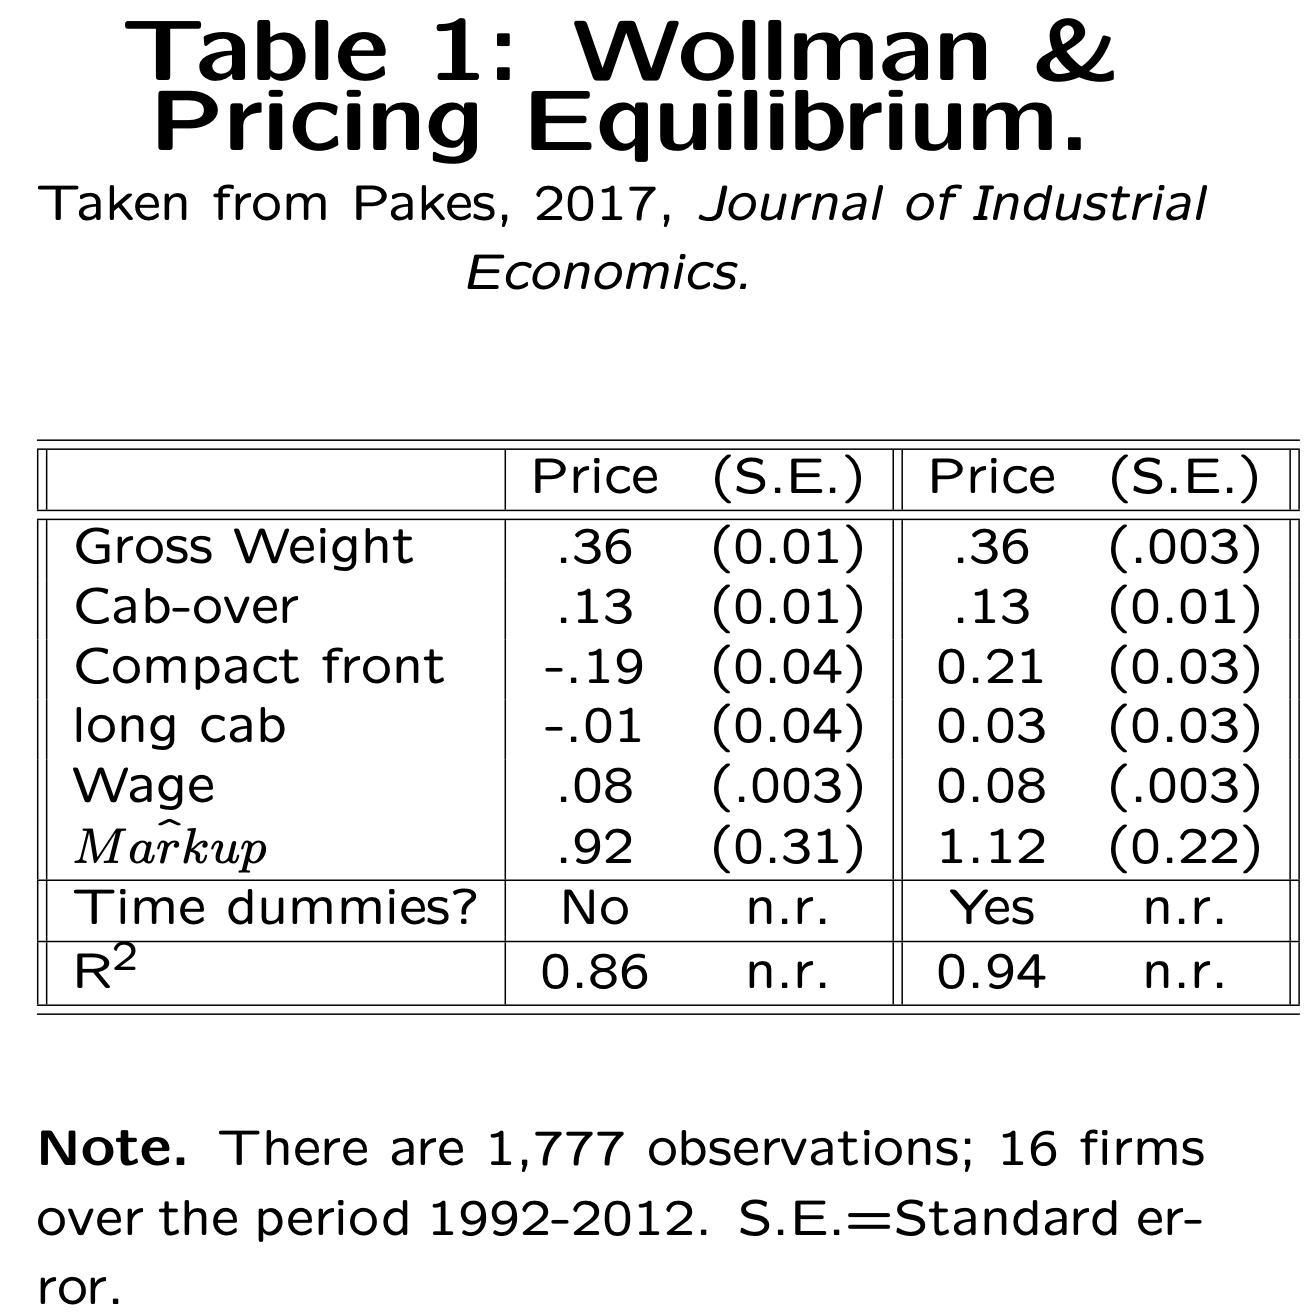
\includegraphics[height=0.9\textheight]{./resources/wollman_regression.png}
\end{center}
\end{frame}

\begin{frame}{Single Model Regressions}
These are somewhat reassuring:
\begin{itemize}
\item $\lambda\approx 1$ for multiproduct-oligopoly
\item Fit is pretty good $R^2 > 0.8$ and $R^2 > 0.5$ for within vehicle regressions (not shown).
\item As a behavioral model, multiproduct demand estimation seems successful.
\item But, do we know that an alternative $\mathcal{H}(\kappa)$ would have a $\lambda \neq 1$ or a lower $R^2$, and if so how low before we can ``reject'' the model?
\end{itemize}
\end{frame}

\begin{frame}{Goodness of Fit Tests}
Another idea (Bonnet and Dubois, Rand 2010) runs the following regression:
\begin{align*}
\log \left( p_{jt} - \eta_{jt}(\mathbf{p},\mathbf{s},\widehat{\theta}_2,\kappa) \right) &= h_s(x_{jt}, \alert{w_{jt}},\theta_3) + \omega_{jt}
\end{align*}
\begin{itemize}
\item Run a regression for each $\kappa$ and obtain $Q(\kappa)=\sum_{jt} \widehat{\omega}_{jt}^2$
\item Employ the \alert{non nested test} of Rivers and Vuong (2002). Why?
\item Working out the distribution of $Q(\kappa_1) - Q(\kappa_2)=T(\kappa_1,\kappa_2)$ is the hard part.
\item Also this is OLS (or NLLS) and there are no instruments or \alert{exclusion restrictions} for the supply side. Presumably we could add some and do GMM? (I think this is the ``formal'' test of Villas Boas (ReStud 2007)).
\end{itemize}
\end{frame}

\begin{frame}{Recap}
\small
So far three approaches to exploit $ E[\omega_{jt} | x_{t},w_{t},z_{t}]=0$
\begin{enumerate}
\item Put the markup on RHS and instrument for it to test $\lambda=1$
\begin{align*}
 p_{jt} &= h_s(x_{jt}, \alert{w_{jt}},\theta_3) + \lambda \cdot \eta_{jt}\left(\mathbf{p},\mathbf{s},\widehat{\theta_2},\kappa \right)+  \omega_{jt}
\end{align*}
\item Put the markup on LHS assuming $\lambda=1$ and test goodness of fit of supply equation
\begin{align*}
 p_{jt} -\eta_{jt}\left(\mathbf{p},\mathbf{s},\widehat{\theta_2},\kappa \right)&= h_s(x_{jt}, \alert{w_{jt}},\theta_3) +  \omega_{jt}
\end{align*}
\item Estimate supply and demand simultaneously $[\theta_1,\theta_2,\theta_3]$ and compare goodness of fit for different $\kappa$.
\end{enumerate}

\end{frame}

\begin{frame}{Simultaneous Problem: Menu Approach}
Assume two models of conduct (correct: $\kappa_0$) (incorrect: $\kappa_1$)
\begin{align*}
%\label{eq:both_mc}
f(p_{jt} -\eta_{jt}(\kappa_0))= h(x_{jt},w_{jt};\theta_3^0)+\omega_{jt}^{0},\\
f(p_{jt} -\eta_{jt}(\kappa_1))= h(x_{jt},w_{jt};\theta_3^1)+\omega_{jt}^{1}.
\end{align*}
Write things in terms of the markup difference:
\begin{align*}
p_{jt} -\eta_{jt}(\kappa_1)= h(x_{jt},w_{jt};\theta_3)+ \overbrace{\lambda \cdot  \Delta \eta_{jt}(\mathbf{p},\mathbf{s},\theta,\kappa_0,\kappa_1) +   \omega_{jt}}^{\widetilde{\omega_{jt}}}
\end{align*}
Tempting idea: run the above regression and test if $\lambda=0$.
\begin{itemize}
\item True model $\lambda=0$, alternate model $\lambda \neq 0$.
\item True model will satisfy $E[\widetilde{\omega}_{jt} | x_{t}, \alert{w_{t}}, \alert{v_{t}}]=0$
\item $\eta_{jt}$ is \alert{endogenous}: it depends on everything including $(\xi,\omega)$.
\end{itemize}
\end{frame}


\begin{frame}{A subtle solution}
\begin{itemize}
\item Berry Haile 2014 tell us we need \alert{marginal revenue shifters} to act as \alert{exclusion restrictions}.
\item Needs to be uncorrelated with $p_{jt}-\eta_{jt}(\kappa_0)$ but correlated with $p_{jt}-\eta_{jt}(\kappa_1)$
\begin{itemize}
\item If my marginal cost is correlated with marginal costs of other products or ``closeness of competitors'', I've got the wrong conduct assumption!
\end{itemize}
\item We need an instrument for $\Delta \eta_{jt}(\mathbf{p},\mathbf{s},\theta,\kappa_0,\kappa_1)$
\begin{itemize}
\item Maybe not so hard since it is basically a function of everything.
\item Cannot have a direct effect on $mc_{jt}$ (exclusion restriction).
\end{itemize}
\end{itemize}
\end{frame}



\begin{frame}{Backus, Conlon, Sinkinson (2020)}
What would a really good instrument look like?
\begin{itemize}
\item Chamberlain (1987) style optimal IV for $\kappa_{fg}$ would be $E\left[\frac{\partial \eta_{jt}(\theta_2,\mathbf{s},\mathbf{p},\kappa)}{\partial \kappa_{fg}} | x_{t}, w_{t}, v_{t}\right]$
\begin{itemize}
\item But infeasible without knowledge of $(\kappa,\xi,\omega)$!
\item We could try to recover the infeasible estimate and project it onto $(x_t,w_t,v_t)$ (note: lack of $j$ subscripts!)
\end{itemize}
\item Menu approach: could look at discrete analogue: $E\left[\Delta \eta_{jt}(\kappa_1,\kappa_0,\theta_2,\mathbf{s},\mathbf{p}) | x_{t}, w_{t}, v_{t}\right]$
\begin{itemize}
\item I would need to know $\kappa_1,\kappa_0$.
\item Still infeasible but could run a first-stage regression
\end{itemize}
\end{itemize}
\end{frame}



\begin{frame}{Backus, Conlon, Sinkinson (2020)}
What would a really good instrument look like?
\begin{itemize}
\item Chamberlain (1987) style optimal IV for $\kappa_{fg}$ would be $E\left[\frac{\partial \eta_{jt}(\theta_2,\mathbf{s},\mathbf{p},\kappa)}{\partial \kappa_{fg}} | x_{t}, w_{t}, v_{t}\right]$
\begin{itemize}
\item But infeasible without knowledge of $(\kappa,\xi,\omega)$ so we take expectation over exogenous variables.
\item We could try to recover the infeasible estimate and project it onto $(x_t,w_t,v_t)$ (note: lack of $j$ subscripts!)
\end{itemize}
\item Menu approach: could look at discrete analogue: $E\left[\Delta \eta_{jt}(\kappa_1,\kappa_0,\theta_2,\mathbf{s},\mathbf{p}) | x_{t}, w_{t}, v_{t}\right]$
\begin{itemize}
\item I would need to know $\kappa_1,\kappa_0$.
\item Still infeasible but could run a first-stage regression
\end{itemize}
\end{itemize}
\end{frame}


\begin{frame}{Backus, Conlon, Sinkinson (2020)}
\footnotesize
Our procedure ((1)+(2) can be done separately)
\begin{enumerate}
\item Run OLS to obtain $\widehat{\omega}_1,\widehat{\omega}_2$ for $(\kappa_1,\kappa_2)$
\begin{align*}
\log \left( p_{jt} - \eta_{jt}(\mathbf{p},\mathbf{s},\widehat{\theta}_2,\kappa) \right) = h_s(x_{jt}, w_{jt},\theta_3) + \omega_{jt}
\end{align*}
\item Recover $\Delta \widehat{\eta}_{jt}(\kappa_1,\kappa_2)$ via nonparametric regression/machine-learning
\begin{align*}
\Delta \widehat{\eta_{jt}}(\kappa_1,\kappa_2) = E \left[\Delta \eta_{jt}(\kappa_1,\kappa_2) | z_{t},w_{t},x_{t} \right]
\end{align*}
\item Compute the violations of the moment condition
$Q\left(\kappa^{m}\right)=\left(n^{-1} \sum_{j, t} \hat{\omega}_{j t}^{m} \cdot \widehat{\Delta \eta}_{j t}\right)^{2}$
\item Compute the test statistic: $T=\frac{\sqrt{n}\left(Q\left(\kappa^{1}\right)-Q\left(\kappa^{2}\right)\right)}{\hat{\sigma}}$ and bootstrap the standard error.
\end{enumerate}
Techincally we should \alert{sample split} and estimate the the regressions on \alert{independent} samples.
\end{frame}


\begin{frame}{Backus, Conlon, Sinkinson (2020) [Alternative]}
\begin{align*}
 p_{jt} -\eta_{jt}\left(\mathbf{p},\mathbf{s},\widehat{\theta_2},\kappa \right)&= h_s(x_{jt}, \alert{w_{jt}},\theta_3) +  \omega_{jt}
\end{align*}
\begin{itemize}
\item We can also directly test violations of $E[\omega_{jt} | x_t, v_t, w_t]$ by comparing resulting CUE or GEL (or GMM) objective values.
\item Probably want to include approximate optimal IV $E\left[\frac{\partial \eta_{jt}(\theta_2,\mathbf{s},\mathbf{p},\kappa)}{\partial \kappa_{fg}} | x_{t}, w_{t}, v_{t}\right]$ in instrument set.
\end{itemize}
\end{frame}







\end{document}


\item It turns out that 2SLS analog $E[\Delta \eta_{jt} | x_t, w_t, v_t,Z_{jt}^e]=\widehat{\Delta \eta_{jt}}$ doesn't add much:
\begin{itemize}
\item Markups aren't a linear function of observables.
\item Coefficients are (probably) quite different across products.
\end{itemize}